\documentclass[runningheads]{llncs}
%
\usepackage{amsmath,amssymb,amsfonts}
\usepackage{graphicx}
\graphicspath{{images/}}
\usepackage{textcomp}
\usepackage{xcolor}
\usepackage{booktabs}
\usepackage{array}
\usepackage{url}
\usepackage{tikz}
\usetikzlibrary{arrows.meta,positioning,shapes.geometric}

\setlength{\textfloatsep}{3pt plus 1pt minus 1pt}
\setlength{\intextsep}{3pt plus 1pt minus 1pt}
\setlength{\floatsep}{3pt plus 1pt minus 1pt}
\setlength{\abovecaptionskip}{1pt plus 1pt minus 1pt}
\setlength{\belowcaptionskip}{0pt}
\setlength{\abovedisplayskip}{4pt plus 1pt minus 2pt}
\setlength{\belowdisplayskip}{4pt plus 1pt minus 2pt}

\begin{document}
%
\title{Network-Aware Event Sequence Modeling for User-Behavior and System Log Anomaly Detection}
\titlerunning{Network-Aware Event Sequence Modeling for Log Anomaly Detection}

\author{Thanh Tien Cao\inst{1,2} \and
Tu Hoang Trinh\inst{2}\thanks{Corresponding authors: H. M. Tran (\email{hatm@huflit.edu.vn}) and T. H. Trinh (\email{tht.csec2005@gmail.com}, \email{23dh113972@st.huflit.edu.vn}). Source code, parsed template sequences, transition-graph artifacts, and per-seed metric tables: \protect\url{https://github.com/thtcsec/log-anomaly-tcn-transformer}. Institutional raw HTTP logs are \emph{not} released.} \and
Ha Manh Tran\inst{2}\textsuperscript{*}}
%
\authorrunning{T. T. Cao et al.}

\institute{Industrial University of Ho Chi Minh City, Ho Chi Minh City, Vietnam\\
\email{thanhct25471@pgr.iuh.edu.vn}
\and
Faculty of Information Technology, Ho Chi Minh City University of Foreign Languages - Information Technology, Ho Chi Minh City, Vietnam\\
\email{thanhct@huflit.edu.vn, tht.csec2005@gmail.com, hatm@huflit.edu.vn}}

\maketitle
%
\begin{abstract}
We present a network-aware log anomaly detection pipeline that treats Drain3 templates as vertices of a directed transition graph and each log sequence as a walk on that graph. Walks are scored with explicit transition-probability features (GraphWalk) alongside PCA/SVD, Isolation Forest, a DeepLog-style LSTM, TCN, and a masked Transformer. Classical frequency models remain competitive on HDFS; TCN and DeepLog-style LSTM are nearly tied on BGL; on HUFLIT-Career, compact-vocabulary outlier models remain competitive under heuristic/weak labels. A related HDFS/BGL study has been accepted at VNICT~2026; this paper extends it with GraphWalk scoring, HUFLIT-Career, leakage-aware splits, and deployment analyses.

\keywords{Log anomaly detection \and event-transition network \and Transformer \and Drain3 \and AIOps.}
\end{abstract}

\section{Introduction}
Modern infrastructures generate diverse logs that capture operational state and behavioral patterns. Rule-based detectors age poorly; effective detection requires sequence-level analysis. We model the log stream as a directed event-transition network: Drain3 templates are vertices and successive co-occurrences are edges. A Block ID, time window, or client session is a walk on this graph. On HUFLIT-Career, the transition graph is coupled with a bipartite client--service interaction view. Anomalies are walks that visit rare transitions or deviate quantitatively from normal traversal statistics.

This is an applied evaluation study, not a new detector. The template sequence after Drain3 is an intermediate layer: compact for lightweight baselines, structured for sequence models, and mappable to operational units. We ask: (RQ1)~how does post-Drain3 grouping affect the signal; (RQ2)~how do reconstruction, isolation, graph-walk NLL, next-event prediction, TCN, and masked modeling compare on the same walks; (RQ3)~does the ranking hold from LogHub benchmarks to an institutional web log.

\textbf{Contributions:} (1)~a leakage-aware pipeline that structures logs as walks on directed event-transition (and client--service) graphs; (2)~\emph{operational} GraphWalk scoring via Laplace-smoothed $P(v\mid u)$, alongside classical and deep branches; (3)~evaluation on HDFS, BGL, and HUFLIT-Career with an IP-disjoint ablation; (4)~deployment trade-offs (F1, latency, explainability) and explicit proxy-label limits.

\paragraph{Relation to prior publication.}
A related HDFS/BGL Drain3--TCN--Transformer study has been accepted for publication at VNICT~2026~\cite{b26}; proceedings are forthcoming. This CSoNet paper extends that report with HUFLIT-Career, explicit transition-graph scoring, grouping/latency/explainability analyses, and clearer label/reproduction limits.

\section{Related Work}
Early methods map logs to count vectors and apply PCA, clustering, or Isolation Forest~\cite{b10,b11,b24}. They are lightweight but ignore event order. Sequential models such as DeepLog~\cite{b1}, LogAnomaly~\cite{b13}, and LogRobust~\cite{b14} predict or score event trajectories with LSTM/RNN variants; PLELog~\cite{b15} reduces label cost via probabilistic estimation. Drain/Drain3~\cite{b3} provide fast online parsing; LogPPT~\cite{b7} improves few-shot parsing. Transformer approaches (LogBERT~\cite{b2}, surveys~\cite{b16}) use masked event modeling; LLM/prompt methods (LogPrompt~\cite{b8}, LogGPT~\cite{b9}, LogLLM~\cite{b20}, CoLA~\cite{b21}, LogFiT~\cite{b22}, LINEADAPTER~\cite{b23}, LogAction~\cite{b25}) improve semantics at higher latency.

\textbf{Graph-based log anomaly detection.} LogGD~\cite{b27} converts sequences into graphs and applies GNNs. Logs2Graphs~\cite{b28} builds attributed directed weighted graphs for unsupervised detection. Our GraphWalk branch is intentionally lighter: a first-order Markov transition graph with NLL and fusion features, not a learned GNN embedding.

\begin{table}[htbp]
\caption{Methodology groups and gaps addressed here}
\centering
\scriptsize
\setlength{\tabcolsep}{2.5pt}
\begin{tabular}{lp{2.0cm}p{2.8cm}p{2.8cm}}
\toprule
\textbf{Group} & \textbf{Rep.} & \textbf{Limitation} & \textbf{This work} \\
\midrule
Statistical & PCA, IF~\cite{b10,b11} & No ordering & Unified baselines \\
Sequential & DeepLog~\cite{b1} & Seq.\ bottleneck & Parallel TCN \\
Transformer & LogBERT~\cite{b2} & Parser-sensitive & Decoupled parse/group/score \\
Graph & LogGD~\cite{b27}, Logs2Graphs~\cite{b28} & Heavy GNN stacks & Lightweight Markov GraphWalk \\
LLM & LogGPT~\cite{b9}, LogLLM~\cite{b20} & High latency & Low-latency TCN/Transformer \\
\bottomrule
\end{tabular}
\label{tab_related_work}
\end{table}

Gaps we target: missing order in classical methods; sequential bottlenecks; parser coupling; and under-specified grouping for network-style walks. We standardize parse$\rightarrow$group$\rightarrow$score with Drain3, evaluate BoE baselines, GraphWalk, DeepLog-style LSTM, TCN, and Transformer (mean$\pm$std over 5 seeds). Code and per-seed dumps: \url{https://github.com/thtcsec/log-anomaly-tcn-transformer}.

\section{Proposed Methodology}
\subsection{Pipeline Overview}
Input: raw logs $L=\{l_1,\ldots,l_N\}$. Output: anomaly score $a(S)$ per walk $S$ (HDFS: Block ID; BGL: window; HUFLIT: client IP window). Six steps: (1)~collect; (2)~normalize variables; (3)~Drain3 parse to event IDs (vertices $V$); (4)~group into walks on the transition graph; (5)~represent walks as BoE/TF-IDF \emph{and} as GraphWalk transition features \emph{or} raw event sequences; (6)~score with reconstruction, Isolation Forest, GraphWalk NLL, or sequence models (Fig.~\ref{fig_pipeline}).

\begin{figure}[!t]
\centering
\resizebox{0.52\columnwidth}{!}{
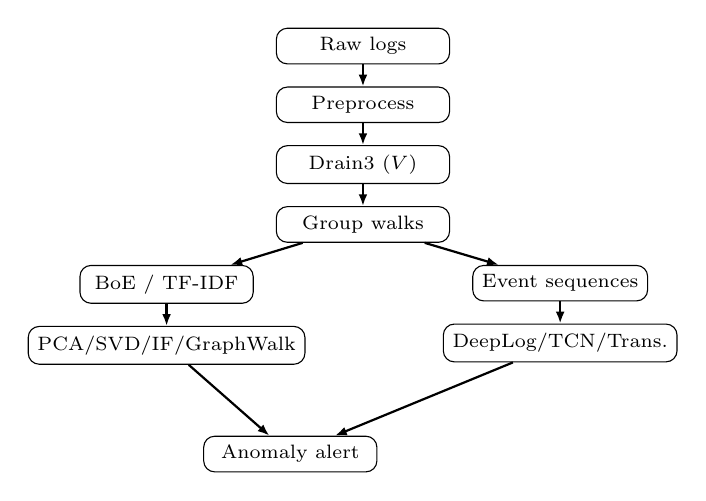
\begin{tikzpicture}[
    node distance=0.28cm and 0.28cm,
    box/.style={rectangle, draw, rounded corners, align=center, minimum width=2.2cm, minimum height=0.42cm, font=\scriptsize},
    arrow/.style={-{Latex[length=1.5mm]}, thick}
]
\node[box] (raw) {Raw logs};
\node[box, below=of raw] (pre) {Preprocess};
\node[box, below=of pre] (parse) {Drain3 ($V$)};
\node[box, below=of parse] (seq) {Group walks};
\node[box, below left=of seq] (vec) {BoE / TF-IDF};
\node[box, below=of vec] (base) {PCA/SVD/IF/GraphWalk};
\node[box, below right=of seq] (bert) {Event sequences};
\node[box, below=of bert] (seqscore) {DeepLog/TCN/Trans.};
\node[box, below right=0.9cm and -1.3cm of base] (score) {Anomaly alert};
\draw[arrow] (raw) -- (pre);
\draw[arrow] (pre) -- (parse);
\draw[arrow] (parse) -- (seq);
\draw[arrow] (seq) -- (vec);
\draw[arrow] (vec) -- (base);
\draw[arrow] (seq) -- (bert);
\draw[arrow] (bert) -- (seqscore);
\draw[arrow] (base) -- (score);
\draw[arrow] (seqscore) -- (score);
\end{tikzpicture}
}
\caption{Parse $\rightarrow$ group walks $\rightarrow$ frequency / GraphWalk / sequence scoring.}
\label{fig_pipeline}
\end{figure}

\subsection{Parsing, Grouping, and Classical Baselines}
Drain3 maps each line to a template via token similarity $Sim(T_1,T_2)$ with threshold $st{=}0.5$ (depth 4). HDFS groups by Block ID; BGL uses non-overlapping $W{=}100$ lines. PCA/TruncatedSVD use BoE counts with reconstruction error and a 95th-percentile threshold on normal training scores ($20$ components). Isolation Forest uses TF-IDF with $200$ trees, fit on normal sequences only. \textbf{Primary IF protocol:} threshold the anomaly score $-\texttt{decision\_function}$ at the 95th percentile of normal training scores (same family as PCA/GraphWalk). Setting \texttt{contamination} to the clipped training anomaly rate is a \emph{label-informed prevalence} calibration and is reported only as a contrast, not as the unsupervised headline.

\subsection{Event-Transition Graph Scoring (GraphWalk)}
\label{sec:graphwalk}
From \emph{normal} training walks we build a directed first-order Markov graph $G=(V,E)$ with Laplace-smoothed transitions
\begin{equation}
P(v\mid u)=\frac{c(u,v)+\alpha}{c(u)+\alpha|V|},\quad \alpha{=}1.
\end{equation}
Each test walk yields mean/worst-edge transition NLL, unseen-edge and novel-node ratios, unique-event ratio, and length. We evaluate GraphWalk mean-NLL (95th-percentile on normal train) and late fusion of $z$-scored GraphWalk NLL with $z$-scored TF-IDF Isolation Forest scores. This makes the network framing an explicit scoring component.

\subsection{Deep Sequence Models}
\textbf{DeepLog-style LSTM:} next-event prediction with a 2-layer LSTM inspired by DeepLog~\cite{b1}, not a bit-exact Spell/full-corpus reproduction. Top-$k$ flags a sequence if any event falls outside the top $K$; NLL uses a 95th-percentile threshold on normal validation. \textbf{TCN:} dilated causal convolutions~\cite{b19} with the same split/scoring protocol. \textbf{Transformer:} masked event modeling~\cite{b2} (mask ratio $0.15$), score $=$ mean MLM loss, 95th-percentile on normal validation.

\textbf{Prefix sizes.} Classical HDFS/BGL baselines use a 500k-line LogHub prefix. DeepLog-style LSTM, TCN, Transformer, and HDFS ablations use a 200k-line prefix (matching public artifacts under \texttt{scripts/} / \texttt{logs/}). Neither setting is the full HDFS\_v1 corpus ($>11$M lines); figures must not be compared directly to $\sim$0.94--0.96 F1 literature numbers under Spell + different protocols~\cite{b1}.

\section{Experimental Setup}
\subsection{Datasets}
HDFS and BGL are from LogHub~\cite{b6,b12}. HUFLIT-Career is a one-month (June 2026) institutional HTTP log; IPs and payloads are hashed. Client IPs are grouping keys only, never features. \textbf{Heuristic/weak labels:} scanner-probe labels come from fixed export rules on \texttt{suspicious\_signals}, not adjudicated SOC ground truth; metrics measure agreement with the heuristic. An IP-disjoint ablation yields PCA F1 $0.6528$ (P~$0.5081$, R~$0.9127$). Dataset statistics (500k prefix for HDFS/BGL counts in Table~\ref{tab_dataset_stats}; deep models use 200k as noted above).

\begin{table}[htbp]
\caption{Dataset statistics after Drain3 (HDFS/BGL: 500k-line prefix)}
\centering
\scriptsize
\begin{tabular}{lccc}
\toprule
\textbf{Metric} & \textbf{HDFS} & \textbf{BGL} & \textbf{HUFLIT} \\
\midrule
Raw lines & 500,000 & 500,000 & 119,516 \\
Grouping & Block ID & $W{=}100$ & Client IP ($W{=}10$) \\
Sequences & 36,305 & 5,000 & 25,049 \\
Normal / anom. & 34,558 / 1,747 & 2,657 / 2,343 & 24,549 / 500 \\
Templates & 137 & 198 & 6 \\
\bottomrule
\end{tabular}
\label{tab_dataset_stats}
\end{table}

\textbf{Splits and thresholds.} Unsupervised scorers train on normal sequences only. HDFS/BGL: 70/30 (classical) or 60/20/20 (neural). Thresholds use the 95th percentile of normal validation/training scores; test labels are never used for $\tau$. Seeds $\{21,42,84,123,777\}$. Hardware: i7-13620H, RTX~4050 6GB, 16GB RAM, Ubuntu 22.04, PyTorch 2.0. Metrics: Precision, Recall, F1 (primary).

\section{Results and Discussion}
\subsection{Cross-Dataset Comparison}
Table~\ref{tab_cross_dataset}: no single winner across protocols. On HDFS, PCA achieves $0.5711\pm0.0944$ under the 500k classical protocol, whereas DeepLog-style and TCN both obtain $0.4613\pm0.0199$ under the 200k deep-model protocol (identical per-seed top-$k$ decisions). Because the prefix sizes differ, these values should \emph{not} be interpreted as a direct head-to-head ranking. The mini Transformer is weaker ($0.2950\pm0.0693$). On BGL (same 500k classical / 200k deep distinction for baselines vs.\ sequence models), TCN top-$k$ ($0.9826\pm0.0022$) is comparable to DeepLog-style ($0.9820\pm0.0042$), not clearly superior. On HUFLIT-Career, PCA leads F1 ($0.6065\pm0.1426$); percentile IF is $0.465\pm0.015$, close to GraphWalk ($0.455\pm0.018$) and deep NLL ($0.5916\pm0.0096$). Contamination-based IF (label-informed prevalence) reaches $\approx$0.63 and is \emph{not} the unsupervised headline.

\begin{table}[htbp]
\caption{Cross-dataset F1 (mean$\pm$std, 5 seeds). HDFS/BGL classical baselines \& IF: 500k; DeepLog/TCN/Transformer \& GraphWalk: 200k (HUFLIT: full). Bold/underline mark best/second \emph{within} BGL and HUFLIT only---not across HDFS prefix protocols.}
\centering
\scriptsize
\setlength{\tabcolsep}{3pt}
\begin{tabular}{lccc}
\toprule
\textbf{Method} & \textbf{HDFS} & \textbf{BGL} & \textbf{HUFLIT} \\
\midrule
PCA & $0.5711\pm0.0944$ & $0.9217\pm0.0098$ & $\mathbf{0.6065\pm0.1426}$ \\
TruncatedSVD & $0.4540\pm0.1366$ & $0.9356\pm0.0117$ & $0.0659\pm0.1474$ \\
Isolation Forest$^\ddagger$ & $0.0381\pm0.0174$ & $0.0172\pm0.0063$ & $0.4650\pm0.0150$ \\
Transformer (val) & $0.2950\pm0.0693$ & $0.9388\pm0.0080$ & $0.3520\pm0.0304$ \\
DeepLog-style (top-k) & $0.4613\pm0.0199$ & $\underline{0.9820\pm0.0042}$ & $0.0665\pm0.0401$ \\
DeepLog-style (NLL) & $0.3046\pm0.0198$ & $0.9381\pm0.0075$ & $0.5916\pm0.0096$ \\
TCN (top-k) & $0.4613\pm0.0199$ & $\mathbf{0.9826\pm0.0022}$ & $0.0451\pm0.0167$ \\
TCN (NLL) & $0.3042\pm0.0236$ & $0.9474\pm0.0035$ & $\underline{0.5916\pm0.0096}$ \\
GraphWalk (NLL)$^{\S}$ & $0.3082\pm0.0278$ & $0.2328\pm0.0474$ & $0.4547\pm0.0179$ \\
\bottomrule
\end{tabular}
\label{tab_cross_dataset}
\end{table}
{\footnotesize $^\ddagger$All reported IF figures use the 95th-pct.\ threshold on $-\texttt{decision\_function}$ (normal train). $^{\S}$\texttt{logs/graph\_transition\_results.json} (5 seeds). Per-seed HDFS top-$k$ (200k): $0.4865,0.4444,0.4725,0.4382,0.4649$ for both DeepLog-style and TCN.}

\begin{figure}[htbp]
\centering
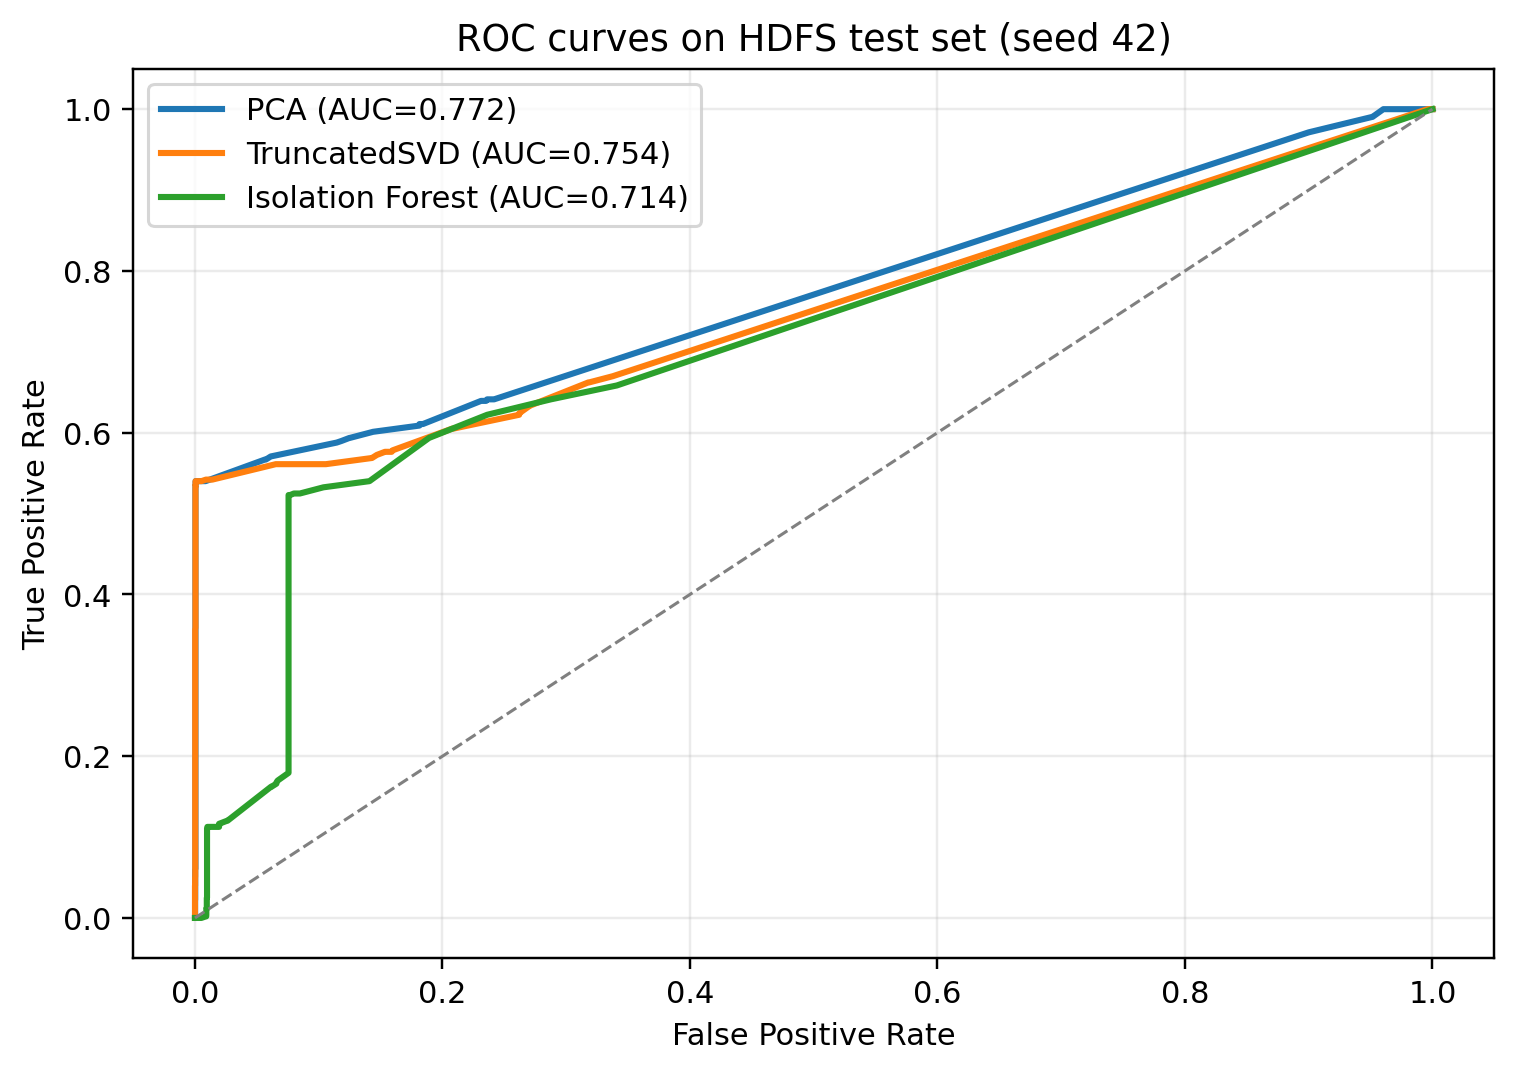
\includegraphics[width=0.98\columnwidth]{roc_curves.png}\\[2pt]
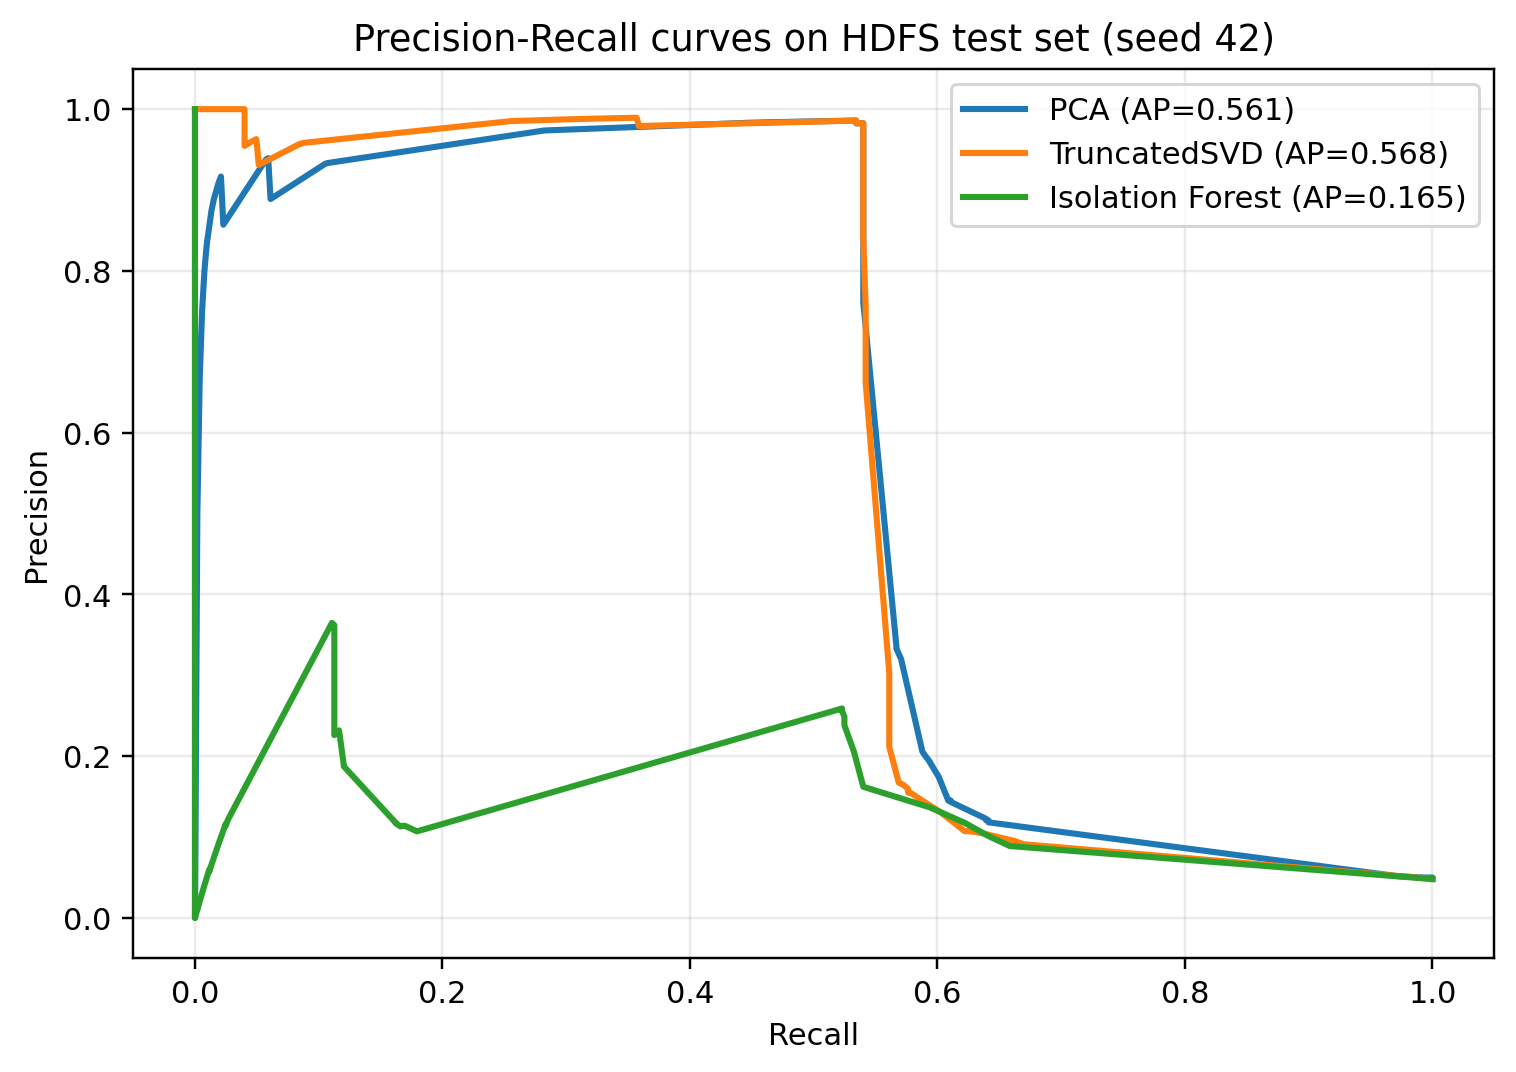
\includegraphics[width=0.98\columnwidth]{pr_curves.png}
\caption{ROC (top) and Precision--Recall (bottom) curves on HDFS, seed 42.}
\label{fig_curves}
\end{figure}

Fig.~\ref{fig_curves}: PCA/SVD separate better than IF on imbalanced HDFS (seed-42 AUROC $0.7722$/$0.7536$/$0.7136$). On HUFLIT, GraphWalk AUROC $0.899\pm0.026$ and percentile IF $0.901\pm0.026$; fusion reaches $0.902\pm0.026$ (Table~\ref{tab_graph_ablation})---a complementary transition-based signal \emph{without} a material aggregate AUROC gain under this setting ($+\approx0.001$ within std).

\begin{table}[htbp]
\caption{HUFLIT graph ablation (5 seeds): transition vs.\ TF-IDF IF vs.\ fusion (95th-pct.)}
\centering
\scriptsize
\begin{tabular}{lcc}
\toprule
\textbf{Scorer} & \textbf{F1} & \textbf{AUROC} \\
\midrule
GraphWalk NLL & $0.455\pm0.018$ & $0.899\pm0.026$ \\
IF TF-IDF (95th pct.) & $0.465\pm0.015$ & $0.901\pm0.026$ \\
Fusion $z$(GW)${+}z$(IF) & $0.465\pm0.016$ & $0.902\pm0.026$ \\
\bottomrule
\end{tabular}
\label{tab_graph_ablation}
\end{table}

\subsection{Isolation Forest Variance}
Under the unified 95th-percentile protocol, IF F1 remains low on HDFS ($0.038\pm0.017$) and BGL ($0.017\pm0.006$) but moderate on Career ($0.465\pm0.015$). Career anomalies are scanner-like in a $\sim$6-template space; HDFS/BGL anomalies often share frequent templates. BGL OR-window labels mix normal and anomalous lines in one bag, collapsing isolation cuts while sequence NLL/top-$k$ still fire locally.

\subsection{Grouping (RQ1) and Ablations}
On BGL 200k, $W\in\{50,100,200\}$ and sliding $W{=}100$/stride $50$ (Table~\ref{tab_grouping}; 3 epochs, 5 seeds): PCA is sensitive to $W$; DeepLog-style/TCN remain robust; sliding yields the strongest sequence F1 (TCN $0.9106\pm0.0181$).

\begin{table}[htbp]
\caption{BGL 200k grouping F1 (mean$\pm$std, 5 seeds)}
\centering
\scriptsize
\begin{tabular}{lccc}
\toprule
\textbf{Config} & \textbf{PCA} & \textbf{DeepLog-style} & \textbf{TCN} \\
\midrule
$W{=}50$ & $0.196\pm0.033$ & $0.832\pm0.023$ & $0.883\pm0.027$ \\
$W{=}100$ & $0.152\pm0.041$ & $0.857\pm0.033$ & $0.886\pm0.018$ \\
$W{=}200$ & $0.477\pm0.084$ & $0.821\pm0.031$ & $0.831\pm0.031$ \\
Sliding $100/50$ & $0.173\pm0.034$ & $0.890\pm0.025$ & $\mathbf{0.911\pm0.018}$ \\
\bottomrule
\end{tabular}
\label{tab_grouping}
\end{table}

On HDFS 200k (seed 42): Drain3 $\theta{=}0.5$ is the sweet spot (25 templates at $0.3$; $2455$ at $0.7$ collapses F1); DeepLog top-$k$ saturates at $K{=}5$--$9$; Transformer mask $r{=}0.15$ is best. Error modes: rare normals as FP; length-driven reconstruction FP; FN when anomalies reuse common templates; template collision under loose $\theta$.

\subsection{Latency and Explainability}
Per-sample latency (batch 1, 1k HDFS samples; Table~\ref{tab_latency}): Drain3 is not the bottleneck; PCA/SVD are fastest; IF is slowest among classical methods; TCN CPU mean ($1.648$~ms) is only $\approx$5.5\% below DeepLog-style ($1.743$~ms)---not a large latency leap. Qualitative TCN mismatches (actual vs.\ top-3 predicted templates + NLL) help operators localize events (e.g., BGL TLB error vs.\ expected kernel transitions).

\begin{table}[htbp]
\caption{Per-sample latency (ms), batch 1, 1k HDFS samples}
\centering
\scriptsize
\setlength{\tabcolsep}{3pt}
\begin{tabular}{lcccc}
\toprule
\textbf{Branch} & Mean & p95 & p99 & Thrpt \\
\midrule
Drain3 (1 line) & 0.007 & 0.010 & 0.023 & 147k/s \\
PCA & 0.063 & 0.153 & 0.219 & 16k/s \\
IF & 4.944 & 9.015 & 11.40 & 202/s \\
DeepLog CPU/GPU & 1.743/0.489 & 2.086/0.798 & 2.407/0.962 & 574/2.0k \\
TCN CPU/GPU & 1.648/0.455 & 2.096/0.780 & 2.609/0.950 & 607/2.2k \\
Transformer CPU/GPU & 2.395/2.916 & 2.966/4.323 & 3.267/4.889 & 418/343 \\
\bottomrule
\end{tabular}
\label{tab_latency}
\end{table}

\textbf{Threats:} lab/campus logs without full SOC triage; domain shift; heuristic HUFLIT labels; Drain3 $\theta$ and grouping dominate F1; mini Transformer under-tuned; DeepLog-style numbers are 200k-prefix protocol matches, not full-corpus reproductions; VNICT~2026~\cite{b26} overlaps the HDFS/BGL backbone (accepted; proceedings forthcoming).

\section{Conclusion}
We evaluated a Drain3 pipeline that uses an event-transition graph (GraphWalk) alongside classical and deep scorers. No branch dominates: PCA remains competitive under the classical HDFS protocol; TCN and DeepLog-style are nearly tied on BGL; PCA leads under Career weak labels, with GraphWalk providing complementary transition signal without material AUROC gain in fusion. Choose scorers by vocabulary size, walk length, and label semantics. Future work: gold SOC labels, GNN embeddings, and matched-prefix HDFS protocols.

\begin{thebibliography}{00}
\scriptsize
\setlength{\itemsep}{0pt}
\setlength{\parskip}{0pt}
\bibitem{b1} M. Du et al., ``DeepLog,'' in \textit{Proc. ACM CCS}, 2017.
\bibitem{b2} H. Guo et al., ``LogBERT,'' in \textit{Proc. IJCNN}, 2021.
\bibitem{b3} P. He et al., ``Drain,'' in \textit{Proc. IEEE ICWS}, 2017.
\bibitem{b4} A. Vaswani et al., ``Attention Is All You Need,'' in \textit{Proc. NeurIPS}, 2017.
\bibitem{b6} J. Zhu et al., ``Tools and Benchmarks for Automated Log Parsing,'' in \textit{Proc. ICSE}, 2019.
\bibitem{b7} V. H. Le and H. Zhang, ``Log Parsing with Prompt-based Few-shot Learning,'' in \textit{Proc. ICSE}, 2023.
\bibitem{b8} T. Zhang et al., ``LogPrompt,'' in \textit{Proc. IJCNN}, 2023.
\bibitem{b9} X. Han et al., ``LogGPT,'' in \textit{Proc. IEEE BigData}, 2023.
\bibitem{b10} V. Chandola et al., ``Anomaly Detection: A Survey,'' \textit{ACM Comput. Surv.}, 2009.
\bibitem{b11} F. T. Liu et al., ``Isolation Forest,'' in \textit{Proc. IEEE ICDM}, 2008.
\bibitem{b12} J. Zhu et al., ``Loghub,'' in \textit{Proc. IEEE ISSRE}, 2023.
\bibitem{b13} W. Meng et al., ``LogAnomaly,'' in \textit{Proc. IJCAI}, 2019.
\bibitem{b14} X. Zhang et al., ``Robust Log-Based Anomaly Detection on Unstable Log Data,'' in \textit{Proc. ESEC/FSE}, 2019.
\bibitem{b15} L. Yang et al., ``Semi-Supervised Log-Based Anomaly Detection via Probabilistic Label Estimation,'' in \textit{Proc. ICSE}, 2021.
\bibitem{b16} M. Landauer et al., ``Deep Learning for Anomaly Detection in Log Data: A Survey,'' \textit{Mach. Learn. Appl.}, 2023.
\bibitem{b17} I. Loshchilov and F. Hutter, ``Decoupled Weight Decay Regularization,'' in \textit{Proc. ICLR}, 2019.
\bibitem{b19} S. Bai et al., ``An Empirical Evaluation of Generic Convolutional and Recurrent Networks for Sequence Modeling,'' \textit{arXiv:1803.01271}, 2018.
\bibitem{b20} W. Guan et al., ``LogLLM,'' \textit{arXiv:2411.08561}, 2024.
\bibitem{b21} X. Zhu et al., ``CoLA,'' \textit{Proc. VLDB Endow.}, 2025.
\bibitem{b22} C. Almodovar et al., ``LogFiT,'' \textit{IEEE Trans. Netw. Service Manag.}, 2024.
\bibitem{b23} X. Liu et al., ``LINEADAPTER,'' preprint, 2025.
\bibitem{b24} B. Yu et al., ``Deep Learning or Classical Machine Learning? An Empirical Study on Log-Based Anomaly Detection,'' in \textit{Proc. ICSE}, 2024.
\bibitem{b25} C. Duan et al., ``LogAction,'' \textit{arXiv:2510.03288}, 2025.
\bibitem{b26} T. T. Cao, T. H. Trinh, and H. M. Tran, ``Application of TCN and Transformer Networks for Log Anomaly Detection in Large-Scale Enterprise and Industrial Networks,'' in \textit{Proc. VNICT}, 2026, EasyChair~\#6979. (Accepted; proceedings forthcoming. Related HDFS/BGL study extended here.)
\bibitem{b27} Y. Xie, H. Zhang, and M. A. Babar, ``LogGD: Anomaly Detection via Graph Neural Networks for Log Sequences,'' in \textit{Proc. APSEC}, 2022.
\bibitem{b28} B. Li et al., ``Logs2Graphs: Unsupervised Anomaly Detection via Attributed Directed Weighted Graphs,'' 2026.
\end{thebibliography}

\end{document}
